\documentclass[professionalfont, 10pt]{beamer} %, handout



%\usepackage{pxfonts}
%\usepackage{eulervm}

%\documentclass[sans,mathserif]{beamer}
%\usepackage{kerkis} % Kerkis roman and sans
%\usepackage{kmath}


%\documentclass[serif, professionalfont]{beamer} %
%\usepackage[T1]{fontenc} % Needed for Type1 Concrete
%\usepackage{concrete}


\usepackage{amsmath}
\usepackage{amsthm}
\usepackage{amsthm,amssymb,amsfonts,amsmath} 
% \usepackage{proof}
\usepackage[mathscr]{eucal}
\usepackage{amssymb,mathtools}
\usepackage{xcolor}
\usepackage{mathrsfs}
\usepackage{enumerate}

\usepackage{tikz}
\usetikzlibrary{shapes.geometric}
\usetikzlibrary{arrows}
\usetikzlibrary{shapes}
\usetikzlibrary{plotmarks}

 
 

\theoremstyle{plain}
\newtheorem{thm}{Theorem}
\newtheorem{remark}{Remark}
\newtheorem{cor}[thm]{Corollary}
 
\theoremstyle{definition}
\newtheorem{df}{Definition}
       
  
\usepackage{epsfig}
%\usepackage{amsmath}
%\usepackage{mathrsfs}
%\usepackage[all]{xy}  
%\usepackage{proof}    %%proof.style file
           

\newcommand{\tcb}[1]{\textcolor{blue}{#1}}
\newcommand{\tcr}[1]{\textcolor{red}{#1}}  
\newcommand{\tcc}[1]{\textcolor{cyan}{#1}}
\newcommand{\tcg}[1]{\textcolor{green}{#1}} 
\newcommand{\tcm}[1]{\textcolor{magenta}{#1}}      

\newcommand{\omt}{\mathop{\curlywedge}}
  
    
\newcommand{\Lra}{\: \Leftrightarrow \:}
\newcommand{\m}[1]{{\mathbf {#1} }}
%\newcommand{\m}[1]{{\mbox{\uppercase {\bf {#1}}}}}
%\newcommand{\N}[1]{{{ \m N_{#1}}}}
\newcommand{\Rl}{ {\mbox{$\mathcal{RL}  $}}}
\newcommand{\Rlc}{ {\mbox{$\mathcal{RL}^C  $}}}
\newcommand{\Ra}{{ \:\; \Rightarrow \:\; }}
%\newcommand{\Ra}{{\mbox{$ \: \Rightarrow \: $}}}
\newcommand{\Rar}{{ \: \Rightarrow \: }}
\newcommand{\La}{{\mbox{$ \: \Leftarrow \: $}}}
\newcommand{\ra}{\rightarrow}
\newcommand{\la}{\leftarrow}
\newcommand{\lra}{\leftrightarrow}
\newcommand{\fa}{\: \forall}
\newcommand{\lan}{(}
\newcommand{\ran}{)}
\newcommand{\rl}{{residuated lattice }}
\newcommand{\rls}{{residuated lattices }}
\newcommand{\T}{\top}
\newcommand{\jn}{\vee}
\newcommand{\mt}{\wedge}
\newcommand{\ror}{\: $ or $ \:}
\newcommand{\rand}{\: $ and $ \:}
\newcommand{\Tg}{\lan \T \ran}
\newcommand{\set}[2]{{\mbox{$ \{ #1 \: | \: #2 \}  $}}}
\newcommand{\ex}{\exists}
\newcommand{\eq}{\approx}
\newcommand{\eqv}{\cong}
\newcommand{\sbs}{\subseteq}
\newcommand{\sps}{\supseteq}
\newcommand{\vr}{{\mbox{$\mathcal{V}$}}}
\newcommand{\Vr}{{\mbox{$ \mathcal{V} \: $ }}}
\newcommand{\vrg}[1]{{\mbox{ $ \mathcal{V}  (\m #1) $}}}
\newcommand{\vs}{\emptyset}
\newcommand{\cov}{\prec}
\newcommand{\rd}{{/}}
\newcommand{\ld}{{\setminus}}
%\newcommand{\qed}{\hfill$\bullet$}
\newcommand{\ol}{\overline}
%\newcommand{\ua}{\hspace{.04in} \uparrow \hspace{-.04in}}
\newcommand{\ua}{\mathop{\uparrow}}
\newcommand{\da}{\hspace{.01in} \downarrow \hspace{-.01in}}
\newcommand{\dm}{\stackrel{\cdot}{-}}
\newcommand{\md}{\stackrel{-}{\cdot}}
\newcommand{\bra}{{\bf \ra}}
\newcommand{\blra}{{\bf \lra}}
\newcommand{\ban}{{\bf \&}}
\newcommand{\bor}{{\bf \nabla}}
\newcommand{\bmt}{{\bf \mt}}
\newcommand{\bjn}{{\bf \jn}}
\newcommand{\bneg}{{\bf \neg}}
\newcommand{\bbot}{{\bf \bot}}
\newcommand{\btop}{{\bf \top}}
\newcommand{\entails}{\vdash}
\newcommand{\TM}{{\mbox{{Turing Machine }}}}
\newcommand{\TMs}{{Turing Machines }}
\newcommand{\MM}{{Minskii Machine }}
\newcommand{\RA}{\Ra}
\newcommand{\rla}{{relation algebra }}
\newcommand{\rlas}{{relation algebras }}
\newcommand{\cv}{ ^{ \cup } }
\newcommand{\cg}{{\rm Cg}}                          %Petar
\newcommand{\var}[1]{{\uppercase \mathcal{{#1}}}}      %Petar
\newcommand{\Lg}{{\mbox{$\mathcal{LG} $}}}             %Partick
\newcommand{\Lgm}{{\mbox{$\mathcal{LG}^- $}}}          %Partick
\newcommand{\phibar}{{\mbox{$\ol \phi\ $}}}         %Partick
\newcommand{\vrm}{{\mbox{$\mathcal{V}^- $}}}           %Partick
\newcommand{\Ya}{\Rightarrow}
\newcommand{\bs}{\boldsymbol}
\newcommand{\cleq}{\preceq}
\newcommand{\hra}{\rightharpoonup}
\renewcommand{\ln}{\mathord{\sim}}
\newcommand{\rn}{\mathord{-}}
\newcommand{\lrh}{\mathop{\leftrightarrow}}
\providecommand{\semsb}{\ensuremath{\mathscr{M}}}
\providecommand{\sem}[1]{\ensuremath{\semsb (#1)}} 
\newcommand{\alhack}{\\[-\normalbaselineskip]\tag*{\qedhere}}
\providecommand{\psetsb}{\ensuremath{\mathscr{P}}}
\providecommand{\pset}[1]{\ensuremath{\psetsb (#1)}} 
\providecommand{\pfin}[1]{\ensuremath{\psetsb_{\text{fin}}(#1)}}

\newcommand{\co}{\mathsf} %fontshape for class operators
\newcommand{\cl}{\mathcal} %fontshape for general classes
\newcommand{\RL}{\va{RL}}
\DeclareMathOperator{\Mod}{Mod}
\newcommand{\bl}{\boldsymbol{\Lambda}}

% Macros for FL
\newcommand{\al}{\alpha}
\newcommand{\sig}{\Sigma}
\newcommand{\lam}{\Lambda}
\newcommand{\gam}{\Gamma}
\newcommand{\del}{\Delta}
\newcommand{\im}{\rightarrow}
\newcommand{\ya}{\rightarrow}
\newcommand{\naraba}{\rightarrow}
\newcommand{\To}{\vdash}
%\newcommand{\lan}{\left(} %not \la
%\newcommand{\ran}{\right)} %not \ra
%\newcommand{\Ya}{\Rightarrow}
\newcommand{\noi}{\noindent}
%\newcommand{\preast}{{\preceq}^{\ast}}
%\newcommand{\prestar}{{\preceq}^{\star}}
\newcommand{\epsi}{\varepsilon}
\newcommand{\e}{\varepsilon}

\newcommand{\p}{\vskip 12pt}
\newcommand{\q}{\vskip 6pt}


\newcommand{\btl}{\lhd}%{\triangleleft}{\blacktriangleleft}
\newcommand{\btr}{\rhd}%{\triangleright}{\blacktriangleright} 
\newcommand{\eb}[1]{\emph{\textcolor{blue}{#1}}}       
\newcommand{\cb}[1]{\textcolor{blue}{#1}} 
\newcommand{\cred}[1]{\textcolor{red}{#1}}        
\newcommand{\ldd}{\mathbin{\bbslash}}
\newcommand{\rdd}{\mathbin{\sslash}}  
\newcommand{\raa}{\mathbin{\leadsto}}    
\newcommand{\RarN}{{\sqsubseteq}}  %{{\mathrel{N}}} 
\newcommand{\RaN}{\mathnormal{\RarN}}

\newcommand{\va}{\mathsf} %fontshape for specific varieties  
\newcommand{\cnv}{u}

\renewcommand{\And}{\text{ \sf and }} %already exists in LaTeX
\newcommand{\Or}{\text{ \sf or }}
\newcommand{\AND}{\text{\sf{AND }}}
\newcommand{\bcdw}{\mbox{\boldmath{$\,\cdot\,$}}}


\renewcommand{\and}{\text{ \sf and }}
\newcommand{\orc}{\text{ \sf or }}
\newcommand{\orb}{\ \overline{\mbox{\sf or}}\ }
\newcommand{\Implies}{\Longrightarrow}
\providecommand{\undsc}{\underline{\phantom{x}}}

\newcommand{\gal}[1]{#1^+}

\newcommand{\force}{\vdash}
\def\hh{\ |\ }
\newcommand{\FL}{\mbox{$\mbox{\bf FL}$}}

\newcommand{\ls}{\setbox0\hbox{$-$}
\mathbin{\hbox{$-$\kern-\wd0\raise2\dp0\hbox{$\cdot$}\kern.3\wd0\lower2\dp0\hbox
{$\cdot$}}}}
\newcommand{\rs}{\setbox0\hbox{$-$}
\mathbin{\hbox{$-$\kern-\wd0\lower2\dp0\hbox{$\cdot$}\kern.3\wd0\raise2\dp0\hbox
{$\cdot$}}}}

\newcommand{\rdo}{\mathop{\mbox{$\bigcirc \! \! \! \! \! \rdd \, $}}}
\newcommand{\ldo}{\mathop{\mbox{$\bigcirc \! \! \! \! \! \ldd \, $}}}

%Lattices 
\providecommand{\MEET}{\ensuremath{\bigwedge}}
\providecommand{\Meet}{\ensuremath{\textstyle\bigwedge\limits}}
\providecommand{\Join}{\ensuremath{\bigvee}}
\providecommand{\meet}{\ensuremath{\wedge}}
\providecommand{\join}{\ensuremath{\vee}}

%Set Theory
\providecommand{\card}[1]{\ensuremath{\left\lvert#1\right\rvert}}
\providecommand{\intersect}{\ensuremath{\cap}}
\providecommand{\Intersect}{\ensuremath{\bigcap}}
\providecommand{\union}{\ensuremath{\cup}}
\providecommand{\UNION}{\ensuremath{\bigcup}}
\providecommand{\Union}{\ensuremath{\textstyle\bigcup\limits}}
%Logic
\providecommand{\iff}{\ensuremath{\Leftrightarrow}}
\providecommand{\implies}{\ensuremath{\Rightarrow}}

%Algebra
\providecommand{\normal}{\ensuremath{\unlhd}}
\providecommand{\embed}{\ensuremath{\hookrightarrow}}%inclusion map
\providecommand{\gen}[1]{\ensuremath{\left<#1\right>}}%Group generated by #1
\providecommand{\idx}[2]{\ensuremath{\left[#1:#2\right]}}%index of #2 in #1
\providecommand{\order}[1]{\ensuremath{\left\lvert#1\right\rvert}}

%Commonly used Sets
\providecommand{\C}{\ensuremath{\mathbb{C}}}%complex
\providecommand{\N}{\ensuremath{\mathbb{N}}}%natural
\providecommand{\Q}{\ensuremath{\mathbb{Q}}}%rationals
\providecommand{\R}{\ensuremath{\mathbb{R}}}%reals
\providecommand{\Z}{\ensuremath{\mathbb{Z}}}%integers
\providecommand{\Zpos}{\ensuremath{\mathbb{Z}^{+}}}%positive integers

%functions
\providecommand{\restrictedto}{\ensuremath{\downharpoonright}}

%Analysis and lineal algebra
\providecommand{\norm}[1]{\ensuremath{\left\lVert#1\right\rVert}}
\providecommand{\vect}{\ensuremath{\vec}}

%Miscellaneous
\providecommand{\abs}[1]{\ensuremath{\left\lvert#1\right\rvert}}
\providecommand{\define}{\ensuremath{\stackrel{\text{\tiny def}}{=}}}

%number theory
\providecommand{\floor}[1]{\ensuremath{\left\lfloor#1\right\rfloor}}
\providecommand{\ceil}[1]{\ensuremath{\left\lceil#1\right\rceil}}

%Miscellaneous shortcuts
\providecommand{\lcm}{\ensuremath{\text{lcm}}}%least common multiple
\providecommand{\st}{\ensuremath{\backepsilon}}

%Presentation dependant
\newcommand{\ccdot}{\bullet}

\newcommand\g[1]{g_{\bf{#1}}}
\newcommand\f[1]{f_{\bf{#1}}}
\newcommand{\gb}{\g{B}}
\newcommand{\gc}{\g{C}}
\newcommand{\fb}{\f{B}}
\newcommand{\fc}{\f{C}}


\usefonttheme[onlymath]{serif}
\usetheme{CambridgeUS} % My favorite!
%with an extra region at the top.
\useoutertheme[subsection=false]{miniframes}%smoothbars}
\definecolor{CrimsonRed}{rgb}{.5882,0,.1804} 
\definecolor{Gold}{rgb}{.6588,.6,.4313}
\definecolor{gold}{HTML}{997316}
\definecolor{Tan}{HTML}{BFB254}%{997316}
%\usecolortheme[named=Tan]{structure} %
%\setbeamercovered{invisible}
%\useoutertheme[right, width=1.8cm]{sidebar}
%\useinnertheme{circles}

\setbeamercolor{palette primary}{fg=CrimsonRed, bg=gold!45!white}
\setbeamercolor{palette sidebar primary}{fg=CrimsonRed} %, bg=gold!20!white}
\setbeamercolor{palette sidebar secondary}{fg=CrimsonRed!90!white}%, bg=gold!18!white}
\setbeamercolor{palette secondary}{fg=CrimsonRed, bg=Gold!30!white}
\setbeamercolor{palette tertiary}{fg=white!80!gold, bg=CrimsonRed}
\setbeamercolor{frametitle}{fg=CrimsonRed, bg=gold!05!white}
\setbeamercolor{title}{fg=gold!40!white, bg=CrimsonRed}
\setbeamercolor{item projected}{bg=Gold!70!white}
 \setbeamercolor{itemize item}{bg=Gold!20!white}
\setbeamertemplate{enumerate items}[default]
\setbeamercolor{block title}{fg=CrimsonRed,bg=gold!35!white}
\setbeamercolor{block body}{fg=black,bg=gold!7!white}
\setbeamercolor{local structure}{fg=Tan!50!white!70!black, }
\setbeamercolor{block title example}{bg=gold!30!white, fg=CrimsonRed}
\setbeamercolor{block body example}{bg=gold!07!white}
%\usecolortheme{sidebartab}

% To remove the navigation symbols from 
% the bottom of slides%
\setbeamertemplate{navigation symbols}{} 
%
\usepackage{graphicx}
%\usepackage{bm}         % For typesetting bold math (not \mathbold)%
%\titlegraphic{\includegraphics[height=1cm]{DU}}
%

\setbeamertemplate{caption}[numbered]
\DeclareMathOperator*{\bigor}{OR}
\newcommand{\bb}[1]{\mathbb {#1}}
\usepackage{setspace}

\title[Algebraic logic presentation 2]{Residuated lattices on $\m M_X$ (part II)\\
Unilinear residuated lattices (part I)}
\author[Xiao Zhuang]{Xiao Zhuang\\
  \small{(joint work with Nick Galatos)} }
\institute[University of Denver]
{University of Denver}
\date{03.07.23}
% \today will show current date. 
% Alternatively, you can specify a date.
% \titlegraphic{\includegraphics[]{}}
%BEAMER HACKS


%Backgroundcolor
%\setbeamercolor{background canvas}{bg=gold!09!white}



\begin{document}


%\begin{frame}[plain]
%\hspace*{1cm}\parbox[t]{\textwidth}{	
%\titlepage
%}
%\end{frame}


\begin{frame}[plain]{}
%\advance\textwidth1.7cm
\hsize\textwidth
\columnwidth\textwidth
\maketitle

\end{frame}

\section{Review}

\begin{frame}{Content of last talk}
    \begin{itemize}
        \item Characterize residuated lattices on $\mathbf{M}_X$:
        The residuated lattices based on $\mathbf{M}_X$ are precisely the ones of the form $\mathbf{R}_{\mathbf{A}, \mathbf{B}}$, where $\mathbf{A}$ is a $\top$-cancellative monoid with zero $\top$ and $\mathbf{B}$ is a semigroup with zero $\bot$, whose multiplication table is one of those in Figure~\ref{f:4tables}.

        \begin{figure}[h]
            \begin{center}
\begin{tabular}{c | c}
 & $\bot$\\
\hline
$\bot$ & $\bot$ 
\end{tabular}
,
\begin{tabular}{c | c c}
 & $\bot$ & $b$\\
\hline
$\bot$ & $\bot$ & $\bot$\\
$b$ & $\bot$ & $b$
\end{tabular}
,
\begin{tabular}{c | c c}
 & $\bot$ & $b$\\
\hline
$\bot$ & $\bot$ & $\bot$\\
$b$ & $\bot$ & $\bot$
\end{tabular}
,
\begin{tabular}{c | c c c}
 & $\bot$ & $b_1$ & $b_2$\\
\hline
$\bot$ & $\bot$ & $\bot$ & $\bot$\\
$b_1$ & $\bot$ & $b_1$ & $\bot$\\
$b_2$ & $\bot$ & $\bot$ & $b_2$ 	
\end{tabular}
\end{center}
            \caption{Four multiplication tables of $Z_R$}
            \label{f:4tables}
        \end{figure}
    \end{itemize}
\end{frame}

\begin{frame}
    \begin{itemize}
        \item The class $\mathsf{URL}_3$ of residuated lattices on $\mathbf{M}_X$ is axiomatized by
        \begin{equation}\tag{URL}\label{axiom_URL}
        u_1 \leq u_2 \text{ or } u_2 \leq u_1 \text{ or } (u_1 \wedge u_2 \leq w \text{ and } z \leq u_1 \vee u_2)
        \end{equation}
        and
        \begin{equation}\tag{$h_3$}\label{axiom_of_finite_height}
            x_1 = x_1 \vee x_2 \text{ or } x_1 \vee x_2 = x_1 \vee x_2 \vee x_3 \text{ or } x_1 \vee x_2 \vee x_3 = x_1 \vee x_2 \vee x_3 \vee x_4
        \end{equation}\pause

        \item The variety $\mathsf{M}$ generated by the class $\mathsf{URL}_3$ is axiomatized by the infinitely many equations
        \begin{align*}
            1 = & \gamma_1(x \backslash y) \vee \gamma_2(y \backslash x) \vee \gamma_3 ((x \wedge y) \backslash z)\\
            1 = & \gamma_4(x \backslash y) \vee \gamma_5(y \backslash x) \vee \gamma_6 (w \backslash (x \vee y))\\
            1 = & \gamma_7((x_1 \vee x_2)\backslash x_1) \vee \gamma_8((x_1 \vee x_2 \vee x_3)\backslash (x_1 \vee x_2))\\
            & \vee \gamma_9((x_1 \vee x_2 \vee x_3 \vee x_4) \backslash (x_1 \vee x_2 \vee x_3)),
        \end{align*}
        where $ \gamma_1, \dots, \gamma_9 \in \Gamma(X)$.\pause

        \item The subdirectly irreducibles in $\mathsf{M}$ are the same as the finitely subdirectly irreducible in $\mathsf{M}$ and they are precisely the non-trivial residuated lattices based on $\mathbf{M}_X$.
    \end{itemize}
\end{frame}

\section{Lattice of subvarieties of $\mathsf{CM_G}$}

\begin{frame}{Uncountably-many subvarieties of $\mathsf{M}$}
There are uncountably many subvarieties of $\mathsf{M}$. \pause
More precisely, we will prove that the variety $\mathsf{CM_G}$ generated by all the residuated lattices of the form $\mathbf{M}_{\mathbf{G}}$, where $\mathbf{G}$ is an abelian group, has uncountably-many subvarieties.
Actually, we give a full description of the subvariety lattice of $\mathsf{CM}_{\mathbf{G}}$.
\pause

The class of commutative $\m M_{\m G}$ is axiomatized by the formula
$$u \leq v \text{ or } v \leq u \text{ or } u \mt v \leq x \text{ or } x \leq u \jn v \text{ or } x(x\ld 1) = 1,$$
which in the bounded case is equivalent to
$$x = \bot \text{ or } x = \top \text{ or } x(x\ld 1) = 1,$$
so the variety $\mathsf{CM}_{\m G}$ generated by the class is axiomatized by $$1 = \gamma_1(u \ld v) \jn \gamma_2(v \ld u) \jn \gamma_3(x \ld (u \jn v)) \jn \gamma_4((u \mt v) \ld x) \jn \gamma_5(x(x\ld 1)),$$
where $\gamma_1, \ldots, \gamma_5 \in \Gamma$.
\end{frame}

\begin{frame}{Sketch of the proof}
    Let $\mathcal{F}$ be a congruence-distributive variety such that $\mathcal{F}_{FSI}$ is a positive universal class.
    We claim that the \textcolor{red}{subvarieties of $\mathcal{F}$} are in bijective correspondence with \textcolor{red}{$\mathsf{HSP_U}$-subclasses of $\mathcal{F}_{FSI}$}, where the correspondence is given by 
    \textcolor{blue}{$\mathcal{V} \mapsto \mathcal{V}_{FSI}$ and $\mathcal{K} \mapsto \mathsf{HSP}(\mathcal{K})$}.\pause
    \begin{block}{Isomorphism (1)}
        The lattice of subvarieties of $\mathsf{CM}_{\mathbf{G}}$ is isomorphic to the lattice of  $\mathsf{HSP_U}$-classes of FSI's in $\mathsf{CM}_{\mathbf{G}}$, which are $\mathsf{HSP_U}$-classes of algebras of the form $\m{M}_{\m{G}}$, where $\m{G}$ is an abelian group.
    \end{block}
    \pause
    Instead of \textcolor{red}{$\mathsf{HSP_U}$-classes}, we are interested in \textcolor{red}{$\mathsf{ISP_U}$-classes} of algebras of the form $\m{M}_{\m{G}}$, where $\m{G}$ is an abelian group.\pause
    We can show \textcolor{red}{$\mathsf{ISP_U}$-classes of $\m M_{\m G}$} are in bijective correspondence with the \textcolor{red}{$\mathsf{ISP_U}$-classes of abelian groups} (isomorphism (2)), by showing \textcolor{blue}{$\mathsf{IP_U}(\m{M}_{\m{H}})=\mathsf{I}\{\m{M}_{\m{G}}: \m{G} \in \mathsf{P_U}(\m{H})\}$ and $\mathsf{S}(\m{M}_{\m{H}})=\{\m{M}_{\m{G}}:  \m{G} \in \mathsf{S}(\m{H})\}$.}
\end{frame}

\begin{frame}
\frametitle{Isomorphisms}
    \begin{block}{Fact}
        Every algebra is an ultraproduct of its finitely generated subalgebras.
    \end{block}
    \textcolor{red}{$\mathsf{ISP_U}$-classes of abelian groups} are fully determined by their \textcolor{red}{intersection with the class of finitely generated abelian groups} (isomorphism (3)).\pause

    \begin{block}{Fundamental theorem of finitely generated abelian groups}
        Every finitely generated abelian group is isomorphic to exactly one group of the form
        \[
            \mathbb{Z}^m \times (\mathbb{Z}_{p_1^{n_{p_1, 1}}} \times \cdots \times \mathbb{Z}_{p_1^{n_{p_1,m_1}}}) \times \cdots \times (\mathbb{Z}_{p_k^{n_{p_k, 1}}} \times \cdots \times \mathbb{Z}_{p_k^{n_{p_k,m_k}}})  
        \]
        for some $k, m, m_1, \dots, m_k,n_{p_i,j} \in \mathbb{N}$, where $n_{i,j} \geq n_{i,j+1}$ for all suitable $j,j$, and $p_1 < p_2< \dots < p_k < \ldots $ is the listing of all primes.
    \end{block}
    We denote by $\mathcal{FA}$ the set of all groups of this form; also by $f\mathcal{A}$ we denote all the finite algebras in $\mathcal{FA}$ (i.e., where $m=0$).
\end{frame}

\begin{frame}
\frametitle{Isomorphisms}
    Instead of considering intersections of $\mathsf{ISP_U}$-classes of abelian groups with the \textcolor{red}{class of finitely generated abelian groups}, we can instead focus on intersections of $\mathsf{ISP_U}$-classes of abelian groups with \textcolor{red}{$\mathcal{FA}$}.\pause
    In other words, we have established that the \textcolor{red}{subvariety lattice of $\mathsf{CM}_{\mathbf{G}}$} is isomorphic to \textcolor{red}{$\{\mathcal{K} \cap \mathcal{FA} : \mathcal{K} \text{ is an } \mathsf{ISP_U} \text{-class of abelian groups}\}$} (isomorphism (4)), where the order is given by: $\mathcal{K} \cap \mathcal{FA} \leq \mathcal{L} \cap \mathcal{FA}$ iff
    $\mathsf{ISP_U}(\mathcal{K} \cap \mathcal{FA}) \subseteq \mathsf{ISP_U}(\mathcal{L} \cap \mathcal{FA})$.

    In the following, we will write $\mathcal{K}_{ \mathcal{FA}}$ for $\mathcal{K} \cap \mathcal{FA}$.\pause
    \begin{block}{Fact}
        Sets of the form $\mathcal{K}_{\mathcal{FA}}$, where $\mathcal{K}$ is an $\mathsf{ISP_U}$-class of abelian groups are of course closed under $\mathsf{S}$ and are, therefore, downsets in $\mathcal{FA}$, where the order is given by $\m G \leq_{\mathcal{FA}} \m H$ iff $\m G \in \mathsf{S}(\m H)$.
        But unfortunately not all downsets of $\mathcal{FA}$ are of this form.
        (For example ${\downarrow} \{\mathbb{Z}^2\}$ is a downset $\mathcal{FA}$ that is not of the form  $\mathcal{K}_{\mathcal{FA}}$.)
    \end{block}
\end{frame}

\begin{frame}
\frametitle{Isomorphisms}
    \begin{block}{Lemma}
        $\m G \times \mathbb{Z}^r \in \mathcal{K}$ iff $\m G \times \mathbb{Z}^s \in \mathcal{K}$ for $r, s \in \bb{Z}^+$, $\m G \in f\mathcal{A}$ and $\mathcal{K}$ an $\mathsf{ISP_U}$-class of abelian groups.
    \end{block}
    \pause
    For this reason, it makes sense to identify $\m G \times \mathbb{Z}^r$ and $\m G \times \mathbb{Z}^s$ whenever $r$ and $s$ are both non-zero.
    This can be done by considering the subset $\mathcal{FA}' = f\mathcal{A} \cup \{\bb{Z} \times \m G: \m G \in f\mathcal{A}\}$ of $\mathcal{FA}$.
    \pause
    \begin{block}{Corollary}
        The lattice of \textcolor{red}{$\{\mathcal{K}_{\mathcal{FA}}: \mathcal{K} \text{ is a } \mathsf{ISP_U} \text{-class}\}$} is isomorphic to the lattice of \textcolor{red}{$\{\mathcal{K}_{\mathcal{FA}'}: \mathcal{K} \text{ is a } \mathsf{ISP_U} \text{-class}\}$} (isomorphism (5)).
    \end{block}
    \pause
    Clearly, if $\mathcal{K}$ is an $\mathsf{ISP_U}$-class of abelian groups, then $\mathcal{K}_{\mathcal{FA}'}$ is a downset of $\mathcal{FA}'$.
    Unfortunately, still not every downset of $\mathcal{FA}'$ is of this form.
    For example, $\{\bb{Z}_p: p \text{ is prime}\}$ is a downset of $\mathcal{FA}'$, but since $\bb{Z} \in \mathsf{P_U}(\{\bb{Z}_p: p \text{ is prime}\})$, $\{\bb{Z}_p: p \text{ is prime}\}$ is not of the form $\mathcal{K}_{\mathcal{FA}'}$.
\end{frame}

\begin{frame}{$\bb{Z}$-closed downsets}
    We consider the direct power $\bb{N}^\omega$ of countably many copies of the chain $(\mathbb{N}, \leq)$ and its subset $I$ of (not necessarily strictly) decreasing sequences that are eventually zero, such as $(4, 2, 1, 1, 0, 0, \dots)$, $(3, 2, 1, 1, 1, 0, 0, \dots)$ etc.
    We also consider the subset $I^{\oplus \omega}$ of the direct product $\m I^\omega$ of all sequences of elements of $I$ that are eventually the zero sequence; it makes sense to call $\m{I}^{\oplus \omega}$ the \emph{direct sum} of $\omega$ copies of $\m I$.\pause
    
    Now let $\m{P} = \m 2 \times \m I^{\oplus \omega}$, where $\m 2$ is the two element lattice on $\{0,1\}$.\pause
    
    For $a \in P$, we write $a=(a_0; a_1; a_2; \ldots)$, where $a_0 \in \{0, 1\}$ and $a_n \in I$, for $n>0$; we define $exp(a)$ to be the maximum number appearing in it; e.g., $exp(1; 2, 1; 3, 1, 1; 0; 2, 1, 1; 0; \dots)=3$ and $exp(0; 1, 1, 1; 4, 1; 3, 2; 0; \dots)=4$.
    Also, for $T \subseteq P$, we define $exp(T) =\{exp(a): a \in T\}$.
    Similarly we define $primes(a) = \{n \in \bb{N}: a(n) \neq \overline{0}\}$ and $primes(T) = \{n \in \bb{N}: (\exists a \in T)(a_n \neq \overline{0})\}$.
\end{frame}

\begin{frame}
A downset $D$ of $\m{P}$ is said to be \emph{$\bb{Z}$-closed} if for all $a \in P$, 
\begin{center}
$exp(D \cap {\uparrow} a)$ or $primes(D \cap {\uparrow} a)$ is unbounded implies that $a' \in D$,
\end{center}
where $a'$ is obtained from $a$ by making the first coordinate equal to $1$.
We denote the lattice of all $\bb{Z}$-closed downsets of $\m{P}$ by $\mathcal{O}_{\bb{Z}}(\m{P})$.\pause

\begin{block}{Lemma}
    $\mathcal{FA}'$ is isomorphic to $\m P = \m 2 \times \m I^{\oplus \omega}$ (isomorphism (6)).
\end{block}
\pause

Therefore, moving through the isomorphism, we can apply the definitions of $exp$ and $primes$ also to downsets of $\mathcal{FA}'$.
To be more specific, a downset $D$ of $\mathcal{FA}'$ is $\bb{Z}$-closed if for all $\m A \in \mathcal{FA}'$,
\begin{center}
    $exp(D \cap {\uparrow} \m A)$ or $primes(D \cap {\uparrow} \m A)$ being unbounded implies that $\bb{Z} \times \m A \in D$ if $\m A \in f\mathcal{A}$ or $\m A \in D$ if $\bb{Z} \leq \m A$.
\end{center}
\end{frame}

\begin{frame}
\frametitle{Isomorphism between $\{\mathcal{K}_{\mathcal{FA}'}\}$ and $\mathcal{O}_{\bb{Z}}(\m P)$}

\begin{block}{$\{\mathcal{K}_{\mathcal{FA}'}\} \leftrightarrow \mathcal{O}_{\bb{Z}}(\m P)$ (isomorphism (7))}
\begin{itemize}
    \item For all $\mathsf{ISP_U}$-class $\mathcal{K}$, $\mathcal{K}_{\mathcal{FA}'}$ is a $\bb{Z}$-closed downset of $\mathcal{FA}'$.

    \item Every $\bb{Z}$-closed downset $D$ of $\mathcal{FA}'$ satisfies $\mathsf{ISP_U}(D) \cap \mathcal{FA}' = D$
\end{itemize}
\end{block}
\pause
\begin{block}{Theorem}
    The subvariety lattice of $\mathsf{CM}_{\mathbf{G}}$ is isomorphic to $\mathcal{O}_{\mathbb{Z}}(\m P)$.
\end{block}
\pause
\begin{block}{Corollary}
    The variety generated by $\{\m M_{\mathbb{Z}_p}: p \text{ is prime}\}$ has continuum-many subvarieties. 
    Therefore the subvariety lattices of $\mathsf{M_G}$ and of $\mathsf{M}$ have size continuum.
\end{block}

\end{frame}

\section{Constructing $\top$-unital URL}

\begin{frame}{$\top$-unital URL}
    Let $\m R$ be a URL.
    If $\m R$ satisfies the formula
    \[
        u \leq v \text{ or } v \leq u \text{ or } x = u \mt v \text{ or } x(u \jn v) = (u \jn v)x = u \jn v,
    \]
    then we call $\m R$ is $\top$-unital.

    Note if $\m R$ is bounded, being $\top$-unital is equivalent to
    \[
        x = \bot \text{ or } x \top = \top x = \top.
    \]

    $\m M_{\m G}$ is a $\top$-unital URL, but there exists $\m M_X$ being not $\top$-unital.
\end{frame}

\begin{frame}{Finite cyclic monoid}
    Given a finite cyclic monoid $\mathbf{M}$ generated by $a \in M$, there is a smallest natural number $r$, called the \emph{index}, such that $a^r = a^{r+s}$ for some  positive integer $s$; the smallest such $s$ then is called the \emph{period}.
    So $M = \{1, a, \dots, a^r, \dots, a^{r+s-1}\}$ and $|M|=r+s$.\pause
    
    Note that every natural number $n > r$ can be written as $n=r+ms+k$ for unique $m \in \mathbb{N}$ and $0 \leq k <s$; we define $[n]_r^s:= r+k$ for $n \geq r+s$ and $[n]_r^s:= n$ for $0 \leq n < r+s$.
    (We will write $[n]$, when $r,s$ are clear from the context.)
    Then the multiplication on $\m M$ is given by $a^i \cdot a^j =a^{[i+j]_r^s}$.
    In particular, $\{a^r, \dots, a^{r+s-1}\}$ is a subsemigroup of $\m M$ and it is a  group in its own right with identity element $a^t$ such that $t \equiv 0 \, (\text{mod } s)$; so it is isomorphic to $\mathbb{Z}_s$.
\end{frame}

\begin{frame}{$\top$-unital URL: $\m R_{\m M}$}
    We extend the multiplication of $\m M$ to the set $R = M \cup \{\bot, \top\}$ by $\bot x = x \bot = \bot$ for all $x \in R$, and $\top x = x \top = \top$ for all $x \not = \bot$.
    Also we define an order on $R$ by $\bot \leq x \leq \top$ for all $x \in R$ and
    $a^i \leq a^j$ if and only if $j = i+ns$ for some $0 \leq n \leq \lfloor (r+s-1-i)/s \rfloor$, for all $0 \leq i, j \leq r+s-1$.
    It is easy to see that this yields a unilinear lattice order.
    We denote by $\m R_{\m M}$ the resulting lattice-ordered monoid.

    \begin{block}{}
        If $\m M$ is a finite cyclic monoid, then $\mathbf{R}_{\m M}$ is the reduct of a resiudated lattice.
    \end{block}
    \pause

    Actually, we can prove that given a finite cyclic monoid $M$, there are only two lattices over which $\m R_{\m M}$ is a reduct of a residuated lattice.
\end{frame}

\begin{frame}
\begin{figure}[h]
\centering
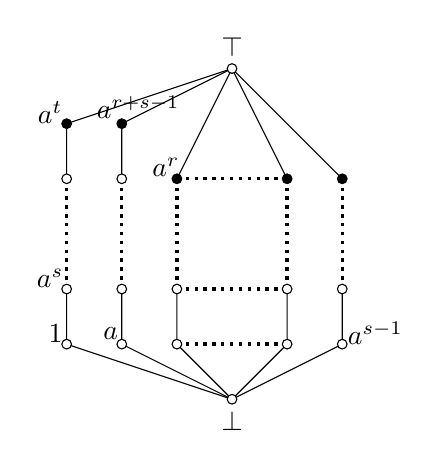
\begin{tikzpicture}[scale = 0.7]
\draw (3, 3) -- (0, 2) -- (0, 1);
\draw [very thick, dotted] (0, 1) -- (0, -1);
\draw (0, -1) -- (0, -2) -- (3, -3);
\draw (3, 3) -- (1, 2) -- (1, 1);
\draw [very thick, dotted] (1, 1) -- (1, -1);
\draw (1, -1) -- (1, -2) -- (3, -3);
\draw (3, 3) -- (2, 1);
\draw [very thick, dotted] (2, 1) -- (2, -1);
\draw (2, -1) -- (2, -2) -- (3, -3);
\draw [very thick, dotted] (2, 1) -- (4, 1);
\draw [very thick, dotted] (2, -1) -- (4, -1);
\draw [very thick, dotted] (2, -2) -- (4, -2);
\draw (3, 3) -- (4, 1);
\draw [very thick, dotted] (4, 1) -- (4, -1);
\draw (4, -1) -- (4, -2) -- (3, -3);
\draw (3, 3) -- (5, 1);
\draw [very thick, dotted] (5, 1) -- (5, -1);
\draw (5, -1) -- (5, -2) -- (3, -3);

\filldraw [color = black, fill = white] (3, 3) circle (2.5pt)
    (3, 3.4) node {$\top$};
\filldraw [color = black, fill = white] (3, -3) circle (2.5pt)
    (3, -3.4) node {$\bot$};
\filldraw [color = black, fill = black] (0, 2) circle (2.5pt)
    (-0.3, 2.2) node {$a^{t}$};
\filldraw [color = black, fill = white] (0, 1) circle (2.5pt);
\filldraw [color = black, fill = white] (0, -1) circle (2.5pt)
    (-0.3, -0.8) node {$a^s$};
\filldraw [color = black, fill = white] (0, -2) circle (2.5pt)
    (-0.2, -1.8) node {$1$};
    
\filldraw [color = black, fill = black] (1, 2) circle (2.5pt)
    (1.3, 2.3) node {$a^{r+s-1}$};
\filldraw [color = black, fill = white] (1, 1) circle (2.5pt);
\filldraw [color = black, fill = white] (1, -1) circle (2.5pt);
\filldraw [color = black, fill = white] (1, -2) circle (2.5pt)
    (0.8, -1.8) node {$a$};
    
\filldraw [color = black, fill = black] (2, 1) circle (2.5pt)
    (1.8, 1.2) node {$a^r$};
\filldraw [color = black, fill = white] (2, -1) circle (2.5pt);
\filldraw [color = black, fill = white] (2, -2) circle (2.5pt);
    
\filldraw [color = black, fill = black] (4, 1) circle (2.5pt);
\filldraw [color = black, fill = white] (4, -1) circle (2.5pt);
\filldraw [color = black, fill = white] (4, -2) circle (2.5pt);
    
\filldraw [color = black, fill = black] (5, 1) circle (2.5pt);
\filldraw [color = black, fill = white] (5, -1) circle (2.5pt);
\filldraw [color = black, fill = white] (5, -2) circle (2.5pt)
    (5.6, -1.8) node {$a^{s-1}$};
\end{tikzpicture}
\qquad
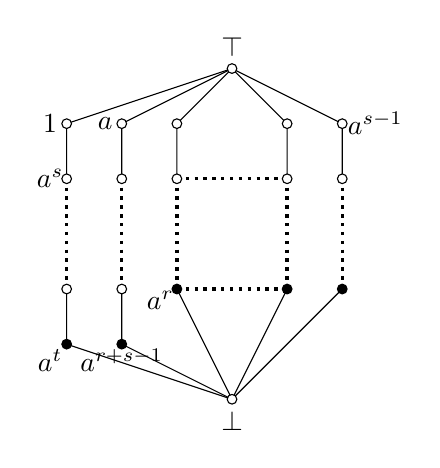
\begin{tikzpicture}[scale=0.70]
\draw (3, 3) -- (0, 2) -- (0, 1);
\draw [very thick, dotted] (0, 1) -- (0, -1);
\draw (0, -1) -- (0, -2) -- (3, -3);
\draw (3, 3) -- (1, 2) -- (1, 1);
\draw [very thick, dotted] (1, 1) -- (1, -1);
\draw (1, -1) -- (1, -2) -- (3, -3);
\draw (3, 3) -- (2, 2) -- (2, 1);
\draw [very thick, dotted] (2, 1) -- (2, -1);
\draw (2, -1) -- (3, -3);
\draw [very thick, dotted] (2, 1) -- (4, 1);
\draw [very thick, dotted] (2, -1) -- (4, -1);
\draw (3, 3) -- (4, 2) -- (4, 1);
\draw [very thick, dotted] (4, 1) -- (4, -1);
\draw (4, -1) -- (3, -3);
\draw (3, 3) -- (5, 2) -- (5, 1);
\draw [very thick, dotted] (5, 1) -- (5, -1);
\draw (5, -1) -- (3, -3);

\filldraw [color = black, fill = white] (3, 3) circle (2.5pt)
    (3, 3.4) node {$\top$};
\filldraw [color = black, fill = white] (3, -3) circle (2.5pt)
    (3, -3.4) node {$\bot$};
\filldraw [color = black, fill = white] (0, 2) circle (2.5pt)
    (-0.3, 2) node {$1$};
\filldraw [color = black, fill = white] (0, 1) circle (2.5pt)
    (-0.3, 1) node {$a^s$};
\filldraw [color = black, fill = white] (0, -1) circle (2.5pt);
\filldraw [color = black, fill = black] (0, -2) circle (2.5pt)
    (-0.3, -2.3) node {$a^t$};
    
\filldraw [color = black, fill = white] (1, 2) circle (2.5pt)
    (0.7, 2) node {$a$};
\filldraw [color = black, fill = white] (1, 1) circle (2.5pt);
\filldraw [color = black, fill = white] (1, -1) circle (2.5pt);
\filldraw [color = black, fill = black] (1, -2) circle (2.5pt)
    (1, -2.3) node {$a^{r+s-1}$};
    
\filldraw [color = black, fill = white] (2, 2) circle (2.5pt);
\filldraw [color = black, fill = white] (2, 1) circle (2.5pt);
\filldraw [color = black, fill = black] (2, -1) circle (2.5pt)
    (1.7, -1.2) node {$a^r$};
    
\filldraw [color = black, fill = white] (4, 2) circle (2.5pt);
\filldraw [color = black, fill = white] (4, 1) circle (2.5pt);
\filldraw [color = black, fill = black] (4, -1) circle (2.5pt);
    
\filldraw [color = black, fill = white] (5, 2) circle (2.5pt)
    (5.6, 2) node {$a^{s-1}$};
\filldraw [color = black, fill = white] (5, 1) circle (2.5pt);
\filldraw [color = black, fill = black] (5, -1) circle (2.5pt);
\end{tikzpicture}
\caption{The two URLs based on a finite cyclic monoid}
\label{fin.cyclicmonid}
\end{figure}
\end{frame}

\begin{frame}
    The divisions on $\m M$ in the two cases are:

    (Left)
    \begin{align*}
    a^i \rightarrow a^j =
    \begin{cases}
        %\top \quad \text{ if } x = \bot, y \in R \text{ or } x \in R, y = \top\\
        %\bot \quad \text{ if } x = \top, y \in R \setminus \{\top\} \text{ or } x \in R \setminus \{\bot\}, y = \bot \text{ or }\\
        \bot & \text{if } j < i \leq r  \text{ or } j< r \leq i \leq r+s-1\\
        a^{j-i} & \text{if } i \leq j < r\\
        a^{j-i+\lfloor \frac{r+s-1+i-j}{s} \rfloor s} & \text{if } i < r \leq j \leq r+s-1\\
        a^k & \text{if }  r \leq i, j, k \leq r+s-1 \text{ and } a^i a^k = a^j.
    \end{cases}
    \end{align*}
    (Right)
    \begin{align*}
    a^i \rightarrow a^j =
    \begin{cases}
       % \top \quad \text{ if } x = \bot, y \in R \text{ or } x \in R, y = \top\\
        %\bot \quad \text{ if } x = \top, y \in R \setminus \{\top\} \text{ or } x \in R \setminus \{\bot\}, y = \bot\\
        a^{j-i} & \text{if } i \leq j \leq r+s-1\\
        a^{j-i+\lceil \frac{i-j}{s} \rceil s} & \text{if } j < i < r \text{ or }  j < r \leq i \leq r+s-1\\
        a^{k-\lfloor \frac{k}{s} \rfloor s} & \text{if } r \leq j < i \leq r+s-1 \text{ and } r \leq k \leq r+s-1\\
                & \qquad \text{ such that } a^i a^k = a^j
    \end{cases}
    \end{align*}
\end{frame}

\begin{frame}{Ordered $2$-cocycles}
    Given a monoid $\mathbf{K}$, a totally-ordered monoid $\mathbf{A}$ and a map $\varphi: \mathbf{K} \rightarrow \m {ResEnd}(\mathbf{A})$, a function $f: K \times K \rightarrow A$ is called an \emph{ordered 2-cocycle} with respective to $\m K, \m A, \varphi$, if it satisfies the following conditions:
    \begin{enumerate}
    \item $f(a_1, a_2)$ is invertible, for all $a_1, a_2 \in K$.
    %, i.e., for all $a_1, a_2 \in A$ there exists $a \in A$ such $a \cdot f(a_1, a_2) = f(a_1, a_2) \cdot a = 1$.

    \item $f(a, 1) = f(1,a)= 1$, for all $a \in K$.

    \item $\varphi_{1_{\mathbf{K}}} = \text{id}_{\mathbf{A}}$ and $\varphi_{a_1 a_2} (b) = f(a_1, a_2) \cdot_{\mathbf{A}} \varphi_{a_1} \varphi_{a_2} (b) \cdot_{\mathbf{A}} f(a_1, a_2)^{-1}$ for all $a_1, a_2 \in K$ and $b \in A$.
    
    \item $f(a_1, a_2 a_3) \varphi_{a_1}(f(a_2, a_3)) = f(a_1 a_2, a_3) f(a_1, a_2)$, for $a_1, a_2, a_3 \in K$.
    \end{enumerate}
\end{frame}

\begin{frame}{$\top$-unital URL: $\m R_{\varphi, f}$}
    Given a cancellative monoid $\mathbf{K}$, a residuated chain $\mathbf{A}$, a map $\varphi: K \rightarrow \m {ResEnd}(\mathbf{A})$ and an ordered 2-cocycle $f: K \times K \rightarrow A$, we  define multiplication on $A \times K$ by 
    \begin{align*}
    (a_1, k_1) \cdot (a_2, k_2) = (a_1 \varphi_{k_1} (a_2) f(k_1, k_2)^{-1}, k_1 k_2)
    \end{align*}
    Also, we extend the multiplication to $R = A \times K \cup \{\bot, \top\}$ by making $\bot$ absorbing for $R$ and $\top$ absorbing for $R \setminus\{\bot\}$,and we define a lattice ordering $\leq$ by: $\bot = \bot < (a, k) < \top = \top$ and
    \[
    (a_1, k_1) \leq (a_2, k_2) \text{ iff } a_1 \leq_{\mathbf{A}} a_2 \text{ and } k_1 = k_2.
    \]
    We denote the resulting algebra by $\mathbf{R}_{\varphi, f}$.
\end{frame}

\begin{frame}
    \begin{figure}
    \begin{center}
    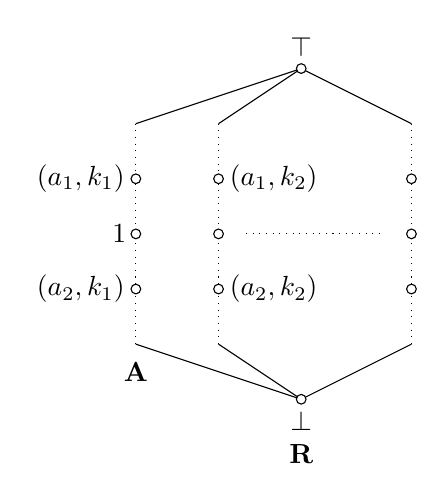
\begin{tikzpicture}[scale=0.70]
        \draw (3, 3) -- (0, 2);
        \draw[dotted] (0, 2) -- (0, -2);
        \draw (0, -2) -- (3, -3);
        \draw (3, 3) -- (1.5, 2);
        \draw[dotted] (1.5, 2) -- (1.5, -2);
        \draw (1.5, -2) -- (3, -3);
        \draw (3, 3) -- (5, 2);
        \draw[dotted] (5, 2) -- (5, -2);
        \draw (5, -2) -- (3, -3);
        \draw[dotted] (2, 0) -- (4.5, 0);

        \draw (0, -2.5) node {$\mathbf{A}$};
        \draw (3, -4) node {$\mathbf{R}$};

        \filldraw [color = black, fill = white] (3, 3) circle(2.5pt)
            (3, 3.4) node {$\top$};
        \filldraw [color = black, fill = white] (3, -3) circle(2.5pt)
            (3, -3.4) node {$\bot$};
        \filldraw [color = black, fill = white] (0, 1) circle(2.5pt)
            (-1, 1) node {$(a_1, k_1)$};
        \filldraw [color = black, fill = white] (0, 0) circle(2.5pt)
            (-0.3, 0) node {$1$};
        \filldraw [color = black, fill = white] (0, -1) circle(2.5pt)
            (-1, -1) node {$(a_2, k_1)$};

        \filldraw [color = black, fill = white] (1.5, 1) circle(2.5pt)
            (2.5, 1) node {$(a_1, k_2)$};
        \filldraw [color = black, fill = white] (1.5, 0) circle(2.5pt);
        \filldraw [color = black, fill = white] (1.5, -1) circle(2.5pt)
            (2.5, -1) node {$(a_2, k_2)$};

        \filldraw [color = black, fill = white] (5, 1) circle(2.5pt);
        \filldraw [color = black, fill = white] (5, 0) circle(2.5pt);
        \filldraw [color = black, fill = white] (5, -1) circle(2.5pt);
    \end{tikzpicture}
    \end{center}
    \caption{A URL based on a semidirect product}
    \label{f: semidirect}
    \end{figure}
\end{frame}

\begin{frame}
    \begin{block}{Theorem}
        If $\mathbf{K}$ is a cancellative monoid, $\mathbf{A}$ is a residuated chain, $\varphi: \mathbf{K} \rightarrow \m {ResEnd}(\mathbf{A})$ is a map, and $f: K \times K \rightarrow A$ is an ordered $2$-cocycle with respect to $\m K$, $\m A$ and $\varphi$, then $\mathbf{R}_{\varphi, f}$ is the reduct of a residuated lattice.
    \end{block}
    \pause

    \begin{block}{Corollary}
        If the ordered $2$-cocycle $f$ is trivial, then $\varphi$ is a monoid homomorphism and $(A \times K, \cdot, (1, 1))$ is a semidirect product of $\m A$ and $\m K$.
        In this case, we denote $\m R_{\varphi, f} = \m A \rtimes^b_{\varphi} \m K$.
    \end{block}
    
\end{frame}

\end{document} 
